\subsection{Process View}
\subsubsection{Activity Diagrams} \label{seq_diag}

\begin{figure}[h!]
\begin{center}
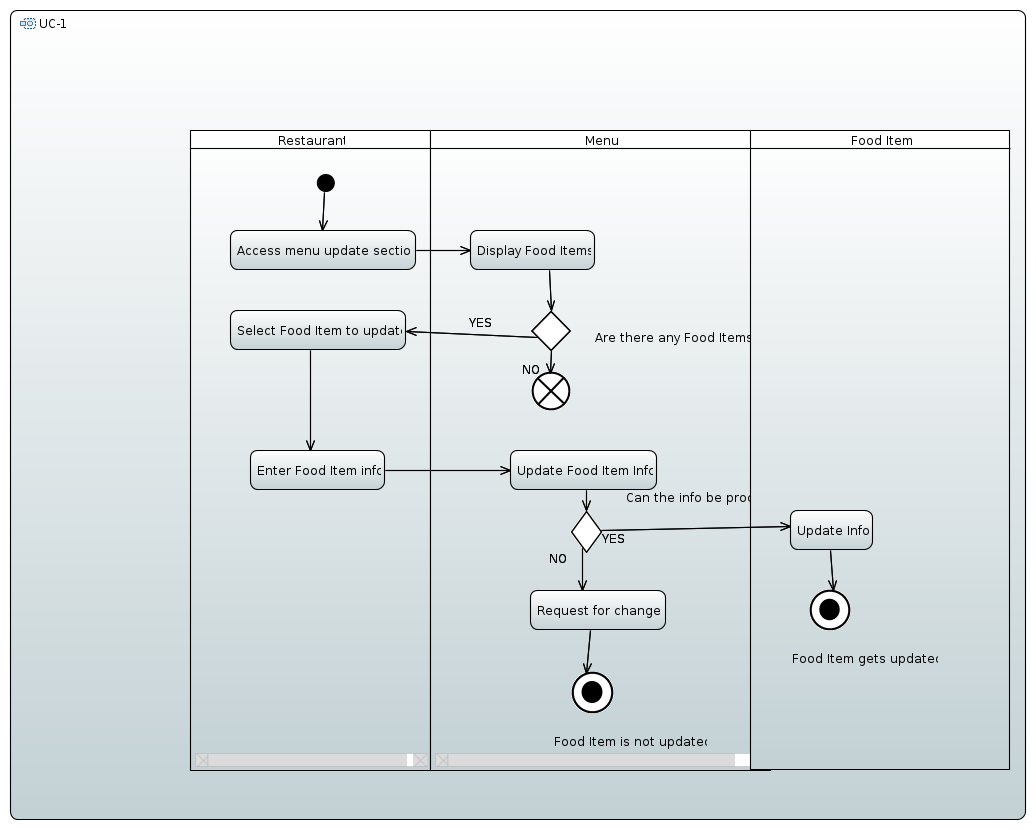
\includegraphics[scale=0.35]{FIGS/UC-1.PNG}
    \caption{Activity Diagram for UC-1}
    \label{fig:act_diag1}
\end{center}
\end{figure}

As described in the first use case and Fig \ref{fig:act_diag1}, the activity will finish unsuccessfully if there are no food items to update or the provided information is wrong, meaning that it is not supported by the system. Otherwise the activity will finish, successfully updating a food item.

\begin{figure}[h!]
\begin{center}
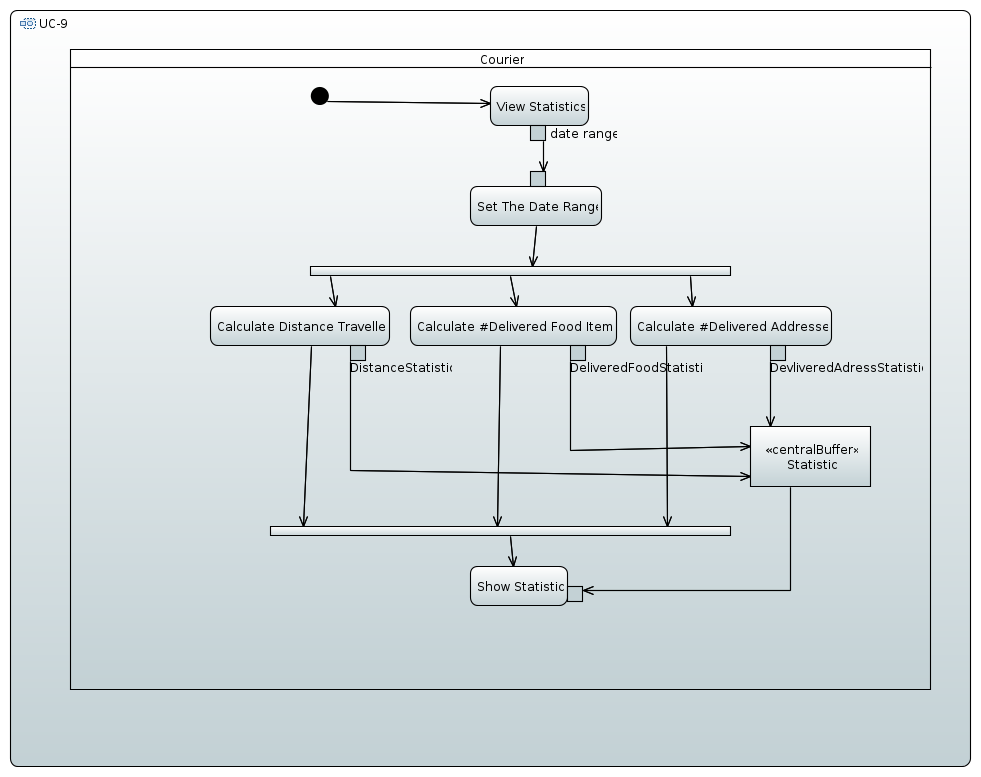
\includegraphics[scale=0.35]{FIGS/UC-9.PNG}
    \caption{Activity Diagram for UC-9}
    \label{fig:act_diag9}
\end{center}
\end{figure}

In another example, Fig \ref{fig:act_diag9} illustrates the activity diagram for use case UC-9. Here, as the courier asks for their statistics, the system starts calculating them concurrently. This concurrency in calculating the statistics will be further reflected in its sequence diagram as well (which we will notice soon).

\subsubsection{Sequence Diagram} \label{seq_diag}

\begin{figure}[h!]
\begin{center}
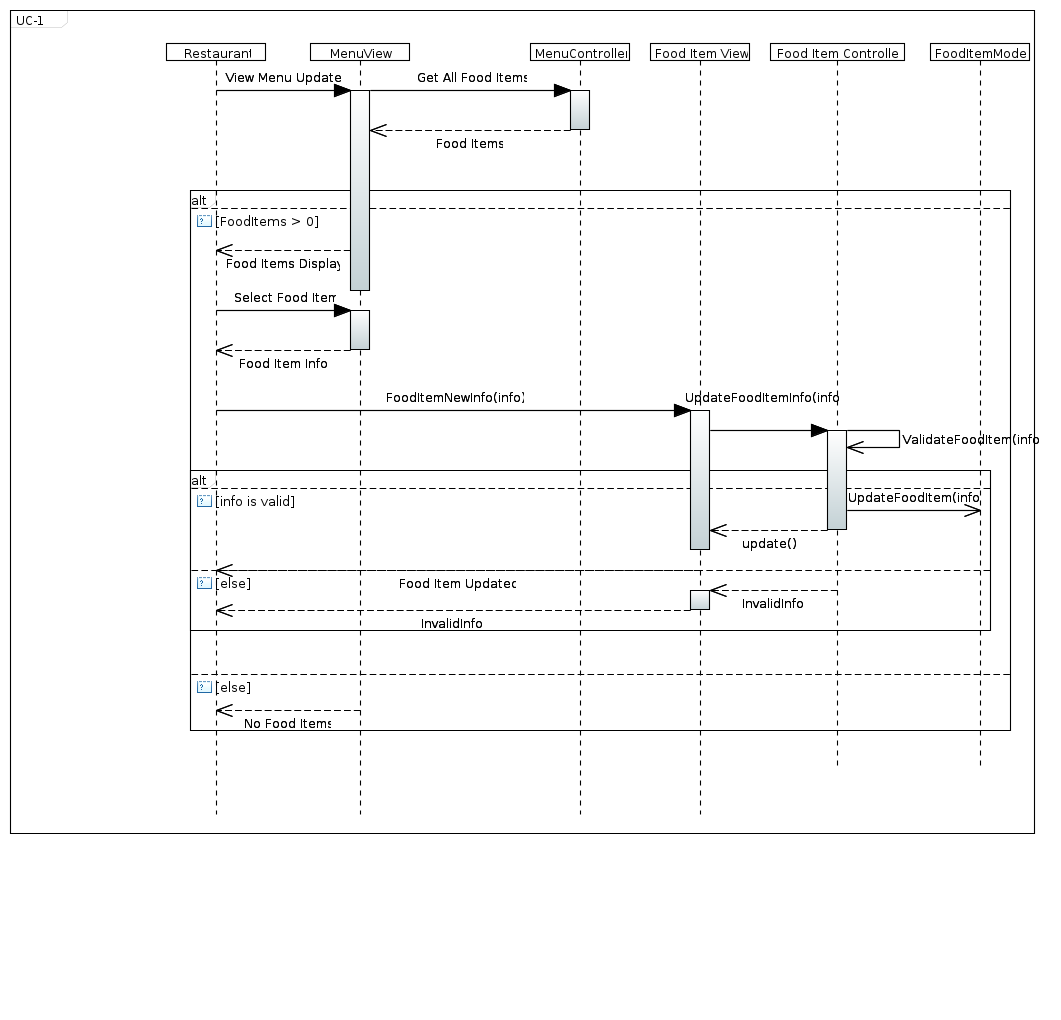
\includegraphics[scale=0.35]{FIGS/UC-11.PNG}
    \caption{Sequence Diagram for UC-1}
    \label{fig:seq_diag1}
\end{center}
\end{figure}

In Fig \ref{fig:seq_diag1}, the MVC style is considered, and access to the different parts of it is controlled. This is, Restaurant can only access the view, not the controller or the model, and the model and controller update the view.

\begin{figure}[h!]
\begin{center}
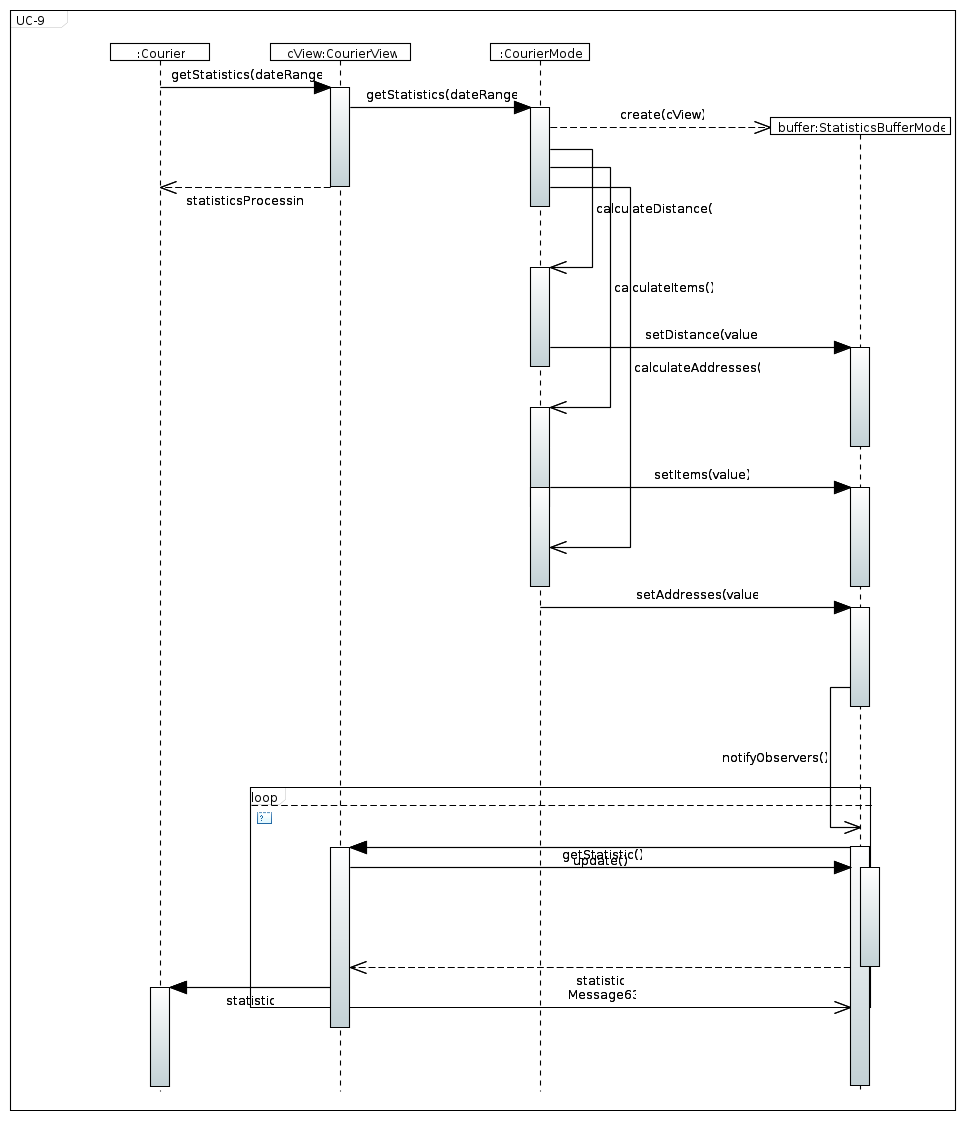
\includegraphics[scale=0.35]{FIGS/UC-91.PNG}
    \caption{Sequence Diagram for UC-9}
    \label{fig:seq_diag9}
\end{center}
\end{figure}

In Fig \ref{fig:seq_diag9}, courier asks for their performance statistics from the system. The model creates a temporary model as the buffer and passes the courier's view to the buffer model for future update. Whenever the buffer calculates all different statistics (in an asynchronous manner), it pushes an update message to the view and the courier's view fetches the statistics from this buffer model and shows them to the user.
